% Copyright (c) 2017-2020 Matematyka dla Ciekawych Świata (http://ciekawi.icm.edu.pl/)
% Copyright (c) 2017-2020 Robert Ryszard Paciorek <rrp@opcode.eu.org>
% Copyright (c) 2020 Krzysztof Lasocki <krz.lasocki@gmail.com>
% 
% MIT License
% 
% Permission is hereby granted, free of charge, to any person obtaining a copy
% of this software and associated documentation files (the "Software"), to deal
% in the Software without restriction, including without limitation the rights
% to use, copy, modify, merge, publish, distribute, sublicense, and/or sell
% copies of the Software, and to permit persons to whom the Software is
% furnished to do so, subject to the following conditions:
% 
% The above copyright notice and this permission notice shall be included in all
% copies or substantial portions of the Software.
% 
% THE SOFTWARE IS PROVIDED "AS IS", WITHOUT WARRANTY OF ANY KIND, EXPRESS OR
% IMPLIED, INCLUDING BUT NOT LIMITED TO THE WARRANTIES OF MERCHANTABILITY,
% FITNESS FOR A PARTICULAR PURPOSE AND NONINFRINGEMENT. IN NO EVENT SHALL THE
% AUTHORS OR COPYRIGHT HOLDERS BE LIABLE FOR ANY CLAIM, DAMAGES OR OTHER
% LIABILITY, WHETHER IN AN ACTION OF CONTRACT, TORT OR OTHERWISE, ARISING FROM,
% OUT OF OR IN CONNECTION WITH THE SOFTWARE OR THE USE OR OTHER DEALINGS IN THE
% SOFTWARE.

\section{Obsługa multimetru}

Multimetr (zwany też miernikiem) to podstawowy przyrząd pomiarowy każdego elektronika. Zgodnie z nazwą posiada wiele funkcji pomiarowych.
Najczęściej są to woltomierz (do pomiaru napięcia stałego \textbf{V$\mathdirectcurrent$} i zmiennego \textbf{V$\sim$}),
amperomierz (do pomiaru natężenia prądu stałego \textbf{A$\mathdirectcurrent$} i zmiennego \textbf{A$\sim$}, potocznie zwanego prądem)
oraz omomierz (do pomiaru rezystancji, \textbf{$\Omega$}). Często multimetr posiada także funkcje:
\begin{itemize}
\item \textbf{Test połączeń} (\textit{continuity mode}), oznaczany symbolem fali dźwiękowej (lub nuty), służy do sprawdzania połączeń elektrycznych.
  Miernik wydaje dźwięk jeśli między sondami pomiarowymi (przewodami) jest połączenie.
\item \textbf{Pomiar diod} (\textit{diode check}), oznaczony symbolem diody \esymbol{diode}, służy do sprawdzania diod i innych elementów półprzewodnikowych.
  Wyświetla spadek napięcia na testowanym złączu półprzewodnikowym.
\item \textbf{Test tranzystorów} (pomiar h\textsubscript{FE}), służący do pomiaru wzmocnienia tranzystora. Najczęściej posiada oddzielne gniazdo
  na mierniku.
\item \textbf{Pomiar pojemności}, oznaczany symbolem \esymbol{capacitor} służy do pomiarów pojemności kondensatorów
\item \textbf{Pomiar temperatury}, ocznaczany symbolem \textbf{$^{\circ}$C}, najczęściej za pomocą termopary (dołączana do miernika).
\end{itemize}

Multimetr zachowuje się tak jak przyrząd pomiarowy, którego funkcjonalność jest aktualnie wybrana. Oznacza to że należy go podłączać
tak samo, jak odpowiednie przyrządy pomiarowe. 

\subsection{Połączenie miernika}
W zależności od modelu, multimetr może posiadać od dwóch do czterech gniazd na przewody. Są to:
\begin{itemize}
\item Masa, oznaczana \textbf{COM} (od słowa \textit{common}). Tutaj podłącza się czarny przewód
\item Wejście pomiarowe dla woltomierza, ozn. symbolem \textbf{V}. Często także jest to wejście omomierza, oznaczone \textbf{$\Omega$},
  oraz testu diod (ozn. symbolem diody \esymbol{diode})
\item Wejście miliamperomierza, oznaczone symbolem \textbf{mA}. Jeżeli Twój miernik posiada trzy wejścia, to najczęściej jest ono
  tym samym wejściem, co wejście woltomierza.
\item Wejście amperomierza, oznaczone symbolem \textbf{A}. Najczęściej również jest obok niego podany maksymalny dopuszczalny prąd
  oraz czas pomiaru.
\end{itemize}

\begin{Ramka}{}\begin{center}
  {\noindent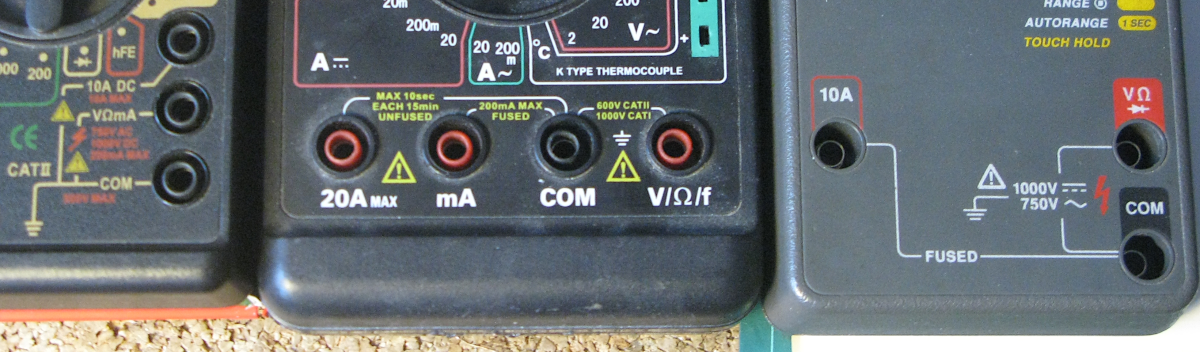
\includegraphics[width=0.99\textwidth,clip=true]{warsztat_elektroniczny/dmm_terminals}}\\
  \small
  Wejścia trzech różnych multimetrów. Pomiędzy wejściami zaznaczone są maksymalne wartości napięcia lub natężenia i informacja o zabezpieczeniach  (``FUSED'') bądź ich braku (``UNFUSED'').\\
  Od lewej: typowy model z trzema wejściami, model z czterema wejściami, model z trzema wejściami (bez miliamperomierza)
\end{center}\end{Ramka}

Przy wyborze multimetru należy zwrócić uwagę na jego wejścia. Modele z czterema wejściami są preferowane (zapewnia to izolację funkcji woltomierza
od amperomierza). Przyrząd musi być też opisany jako ``FUSED'', czyli posiadać bezpiecznik na zakresie miliamperomierza (oraz opcjonalnie,
także amperomierza). Pozwoli to uniknąć uszkodzenia multimetru w wypadku przekroczenia dopuszczalnego natężenia prądu.

\subsection{Woltomierz}
Woltomierz to przyrząd służący do pomiaru napięcia elektrycznego między dwoma punktami. Z tego powodu
\textbf{woltomierz podłączamy równolegle} do elementu, który badamy, lub między dwoma punktami w układzie. Opór woltomierza jest możliwie duży (rzeczywiste
woltomierze mają opór około 1-10 M$\Omega$, woltomierz idealny ma opór nieskoczenie wysoki).

\subsection{Amperomierz}
Amperomierz (tudzież miliamperomierz) służy do pomiaru prądu płynącego w gałęzi obwodu. Z tego powodu
\textbf{amperomierz podłączamy szeregowo} z innymi elementami obwodu. Opór amperomierza jest możliwie mały (idealny amperomierz
ma nieskończenie niski opór).
\\

Podłączenie amperomierza równolegle powoduje zwarcie. Nie należy więc odkładać miernika ustawionego na zakres amperów, szczególnie
w przypadku modeli, które używają tego samego gniazda do pomiaru oporności lub napięcia. Skutki pomyłki mogą być fatalne dla
urządzenia - bezpiecznik się spali.

\subsection{Omomierz}
Omomierz jest przyrządem służącym do pomiaru oporności. Jego zasada działania jest dosyć prosta. Składa się on ze źrodła małego napięcia, które pojawia się na końcówkach przewodów pomiarowych. Gdy przyłożymy sondy do elementu mierzonego, omomierz zmierzy jaki prąd płynie przez element testowany i wyświetli jego opór.
\\

Omomierz w praktyce służy tylko do pomiarów oporników. Trzeba pamiętać o tym, że jeżeli mierzymy element umieszczony w układzie,
to jego oporność będzie zawsze niższa od oczekiwanej. Taki opornik jest połączony równolegle z innymi elementami obwodu o
nieznanym oporze, skąd wynika błąd pomiaru.
Zasadniczo nie wykonuje się za jego pomocą pomiarów oporników we włączonych układach.
\\

Przy pomiarach większych oporników (ponad 100k$\Omega$) należy uważać aby nie dotykać palcami końcówek sond, ponieważ opór Twojego ciała
zaniży pomiar. Lepiej jest położyć opornik na stole i przycisnąć jego nóżki za pomocą końcówek sond.


\subsection{Inne funkcje multimetrów}
Oprócz podstawowych funkcji (pomiaru napięcia, natężenia i oporu)\footnotemark, większość nowoczesnych multimetrów posiada także funkcje pomiaru diod oraz tranzystorów.
\\

Funkcja pomiaru diod jest najczęściej oznaczona symbolem diody półprzewodnikowej (\esymbol{diode}) i korzysta z tej samej pary złącz, co woltomierz i omomierz.
Aby zmierzyć spadek napięcia na diodzie należy dotknąć sondą podłączoną do masy (COM) do katody, a sondą dodatnią do anody. Miernik wyświetli
spadek napęcia na złączu diody. Jeżeli miernik wskazuje wynik poza skalą, może to oznaczać, że polaryzacja diody jest odwrotna (sondy są przyłożone na odwrót).
Może też okazać się, że spadek napięcia na jej złączu jest większy niż zakres pomiaru (który najczęściej wynosi do 2V).
\\

\footnotetext{Mierniki, które posiadają tylko te trzy funkcje nazywane są po angielsku VOM (Volt-ohm-milliammeter). Najczęściej są to mierniki
  analogowe.}

Funkcja pomiaru współczynnika wzmocnienia tranzystora bipolarnego jest z reguły oznaczana \textbf{hFE} (od symbolu $\text{h}_{FE}$ stosowanego do
oznaczenia tej wartości)\footnote{Czasami oznaczanego też jako $\beta$, beta.}. Pomiar tranzystora za pomocą multimetru polega na umieszczeniu jego nóżek w \textbf{odpowiedni sposób} w gnieździe pomiarowym
w multimetrze. Jego emiter, baza oraz kolektor (oznaczane \textbf{E}, \textbf{B} i \textbf{C} odpowiednio) muszą trafić w
otwory w odpowiedniej połowie gniazda (\textbf{PNP} oraz \textbf{NPN} zależnie od typu tranzystora). Trzeba go obrócić tak, żeby emiter trafił do \textbf{E}, baza do \textbf{B} a kolektor do \textbf{C}. Gniadzo jest tak skontstruowane, że
pasują do niego tranzystory o dowolnej kolejności wyprowadzeń. Kolejność dla Twojego tranzystora jest opisana w jego karcie katalogowej.
Po umieszczeniu tranzystora w gnieździe, na ekranie miernika pojawia się wartość jego współczynnika wzmocnienia $\text{h}_{FE}$.
% \todo{umieścić zdjęcie pokazujące to gniazdo}
\\

Niektóre mierniki posiadają także funkcje pomiaru pojemności elektrycznej kondensatora. W zależności od konstrukcji połączenie testowanego
kondensatora odbywa się poprzez umieszczenie go w specjalnym gnieździe na obudowie miernika albo przez podłączenie sond do wyprowadzeń kondensatora. Należy pamiętać
o tym, że trzeba ustawić zakres w podobny sposób jak przy innych pomiarach. Uwaga - \textbf{nie należy mierzyć pojemności naładowanych
  kondensatorów}. Funkcja pomiaru pojemności przydaje się przy sprawdzaniu kondensatorów ceramicznych lub foliowych o pojemnościach od kilku nF do kilkudziesięciu uF. Na kondensatorach elektrolitycznych lub tantalowych (o większych pojemnościach) wartość
pojemności jest z reguły napisana na obudowie. Należy także wybrać kondensator, którego maksymalne dopuszczalne napięcie (też napisane na obudowie)
jest wyższe niż największe możliwe napięcie mogące na nim wystąpić w układzie.

\begin{ProTip}{\normalfont{\strong{Uwaga}}}
  Kondensatory elektrolityczne oraz tantalowe są elementami \textbf{spolaryzowanymi}. Podłączając je, należy o tym pamiętać i podłączać je
  tylko zgodnie z polaryzacją - biegun ujemny do punktu o niższym napięciu, a biegun dodatni do punktu o wyższym napięciu. Na tych kondensatorach jeden
  z biegunów (najczęściej ujemny) jest zaznaczony na obudowie.
  
  \textbf{Uwaga:} Niewłaściwe podłączenie kondensatora może doprowadzić do jego eksplozji.
  Dla własnego bezpieczeństwa nie rób tego – jeżeli jesteś ciekawy jak to wygląda obejrzyj filmik w Internecie.
  Pamiętaj o tym także montując kondensatory w swoich konstrukcjach.
\end{ProTip}

Oprócz opisanych wyżej funkcji, niektóre multimetry mogą mieć także funkcje pomiaru temperatury (poprzez \textbf{termoparę}
lub \textbf{termistor} podłączane do
specjalnego złącza na mierniku) oraz pomiar częstotliwości.

\subsection{Dokonywanie pomiarów}

Zależnie od wielkości fizycznej, którą chcemy zmierzyć, po stroni emiernika, czerwony (dodatni) przewód musi być podłączony do odpowiadającego
mu gniazda. Czarny przewód (ujemny, masa) należy zawsze podłączyć do gniazda \textbf{COM}. Miernik ustawiamy na pomiar danej
wielkości.
\\

Przy wykonywaniu pomiaru nieznanej wartości należy rozpocząć od największego zakresu miernika i stopniowo zmniejszać zakres aż
otrzymamy najdokładniejszy wynik. W przypadku gdy mierzona wartość przekracza aktualny zakres, miernik to zasygnalizuje, najczęściej
wyświetlając ``\textbf{1}'' (po lewej stronie ekranu), lub ``\textbf{OL}'' (\emph{overload}). Oba znaki oznaczają to samo, czyli wartość powyżej zakresu. W takiej sytuacji trzeba przełączyć zakres na większy.
\\

Przy pomiarze \textbf{napięcia} w danym punkcie układu, najczęściej masę miernika (czarną sondę)
podłączamy do masy układu. Drugą sondę (czerwoną) podłączamy do mierzonego punktu. Jeśli chcemy zmierzyć napięcie na jakimś elemencie (np. oporniku),
masą miernika dotykamy do punktu, w którym oczekujemy niższego napięcia, a czerwoną sondą do punktu, w którym oczekujemy
wyższego napięcia. Jeżeli podłączymy sondy odwrotnie, po prostu dostaniemy wynik z przeciwnym znakiem. Woltomierz należy podłączać równolegle.
\\

Przy pomiarze \textbf{natężenia} w danej gałęzi układu należy zachować szczególną ostrożność. Podobnie jak wyżej, zaczynamy pomiar na największym
zakresie miernika. W przeciwieństwie do woltomierza, amperomierz należy podłączyć szeregowo. Ponieważ opór wewnętrzny amperomierza jest bardzo
niski (<1~$\Omega$), trzeba uważać, aby nie zrobić zwarcia.
\\

Pomiaru \textbf{oporności} dokonujemy dotykając końcówkami sond pomiarowych końcówek opornika (lub innego elementu). Dla oporników kolejność przewodów nie ma znaczenia
(opór jest identyczny niezależnie od kierunku płynięcia prądu).
\\

Test połączenia służy do sprawdzania połączeń w układach. Przy wyłączonym zasilaniu dotykamy sondami do punktów, pomiędzy którymi chcemy
sprawdzić połączenie. Jeżeli punkty są połączone, to miernik zasygnalizuje to brzęczykiem. Ta funkcja jest szczególnie przydatna przy sprawdzaniu
prototypów na płytkach stykowych, lub przy sprawdzaniu prawidłowości połączeń w urządzeniu, które diagnozujemy. Jeżeli Twój
multimetr nie ma tej funkcji, to możesz użyć omomierza (bezpośrednie połączenie ma znikomy opór, maksymalnie kilka~$\Omega$).
\\

Tester diod (i innych elementów półprzewodnikowych) pozwala sprawdzić polaryzację złącza półprzewodnikowego w elemencie. W tym celu dotykamy
sondami do obu końców testowanego elementu. Jeżeli ``trafiliśmy'' z polaryzacją sond (podłączyliśmy czarną sondę, COM, do katody, a czerwoną
dodatnią, do anody), to miernik powinien pokazać spadek napięcia na złączu.
W przeciwnym razie pokaże przekroczenie zakresu. Z reguły zakres spadków napięć jakie można w tym trybie zmierzyć jest poniżej 2V, więc
większość diod LED pokaże spadek napięcia poza skalą (niektóre diody LED mogą się bardzo słabo świecić podczas pomiaru jeśli polaryzacja
sond jest prawidłowa).
\\

W niektórych multimetrach test diody jest wspólny z testem połączeń. W takim wypadku, w trybie testu multimetr sygnalizuje
buzzerem sytuację, gdy spadek napięcia jest odpowiednio mały. Oznacza to, że mierzone punkty są ze sobą zwarte
(lub połączone bardzo małym oporem).\\

\begin{ProTip}{\normalfont{\strong{Wskazówka}}}
  W zmontowanym i zasilonym układzie należy dokonywać tylko pomiarów woltomierzem.
  Amperomierz włącza się w szeregowo w badany układ, zatem jego użycie wymaga modyfikacji układu, chyba że układ przewiduje możliwość takiego pomiaru.
  
  Omomierz i pomiar pojemności używa się do pomiarów elementów poza układem,
  jednak pomiar ciągłości (rzadziej oporności) może być wykonywany na wyłączonym układzie celem ustalenia dlaczego ten nie działa.
  Należy wtedy pamiętać o tym, że pomiary omomierzem będą zaniżone z  powodu obecności innych oporów w układzie.
\end{ProTip}
